\documentclass{standalone}
\usepackage{tikz} % Import the tikz package
\usetikzlibrary{automata} % Import library for drawing automata
\usetikzlibrary{positioning} % ...positioning nodes
\usetikzlibrary{arrows} % ...customizing arrows
\tikzset{node distance=2.5cm,
    every state/.style={
        semithick,
        fill=gray!10},
    initial text={},
    double distance=2pt,
    every edge/.style={
        draw,
        ->,>=stealth',
        auto,
        semithick}}
\let\epsilon\varepsilon
\begin{document}
    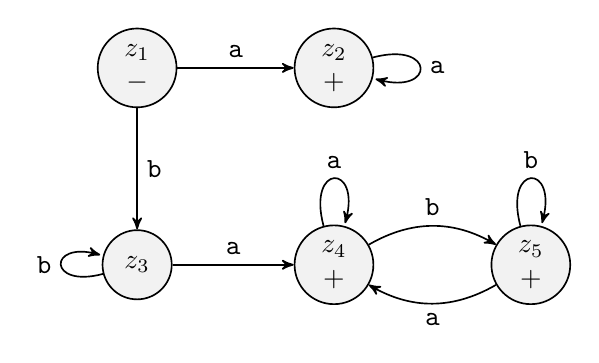
\begin{tikzpicture}
        \node[state,align=center] (z1) {$z_1$\\$-$};
        \node[state,right of=z1,align=center] (z2) {$z_2$\\$+$};
        \node[state,below of=z1] (z3) {$z_3$};
        \node[state,right of=z3,align=center] (z4) {$z_4$\\$+$};
        \node[state, right of=z4,align=center] (z5) {$z_5$\\$+$};

        \draw (z1) edge[] node {\tt a} (z2);
        \draw (z1) edge[] node {\tt b} (z3);
        \draw (z2) edge[loop right] node {\tt a} (z2);
        \draw (z3) edge[loop left] node {\tt b} (z3);
        \draw (z3) edge[] node {\tt a} (z4);
        \draw (z4) edge[loop above] node {\tt a} (z4);
        \draw (z4) edge[bend left] node {\tt b} (z5);
        \draw (z5) edge[bend left] node {\tt a} (z4);
        \draw (z5) edge[loop above] node {\tt b} (z5);
    \end{tikzpicture}
\end{document}